%!TEX root = ../main.tex
%%%%%%%%%%%%%%%%%%%%%%%%%%%%%%%%%%
% Links:
%
% Difficulty:
% Companies: 
%%%%%%%%%%%%%%%%%%%%%%%%%%%%%%%%%%


%\begin{figure}
%	\centering
%	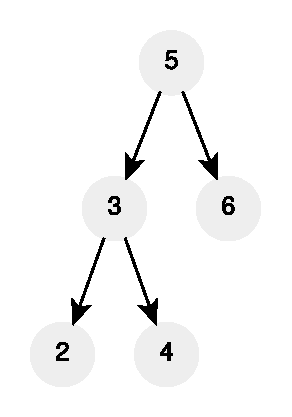
\includegraphics[width=\textwidth]{sources/max_triplet/images/example1}
%	\caption[Sample short cpation]{Sample Caption}.
%	\label{fig:max_triplet:example1}
%\end{figure}

\chapter{Max triplet sum}
\label{ch:max_triplet}
\section*{Introduction}

\section{Problem statement}
\begin{exercise}
\label{example:max_triplet:exercice1}
Write a function that, given an array $I$ of length $n$, returns 
the maximum value obtainable by summing $3$ distinct elements of $I$: $I_i$, $I_j$ and $I_k$ such that
$ 0 \leq i < j < k \leq n-1$ and $ A_i < A_j < A_k $.


	%example1
	\begin{example}
		\label{example:max_triplet:example1}
		\hfill \\
		Given $I = \{2, 5, 3, 1, 4, 9\}$ the function returns $16$.
		The max value of $16$ is obtainable by summing together the 
		elements of $I$ at indices: $0$,$1$ and $5$ : $I_0 + I_1+I_5=2+5+9= 16$.
		
		Notice that there is another way of obtains the max sum of $16$, that is by using the elements
		at indices $2$,$4$ and $5$: $I_2 + I_4+I_5=3+4+9= 16$.
	\end{example}

	%example2
	\begin{example}
		\label{example:max_triplet:example2}
		\hfill \\
		Given $I = \{3,2,1\}$ the function returns $-1$ as there is no valid triplet in $I$.		
	\end{example}
	
		\begin{example}
			\hfill \\
			Given $I = \{1,3,2\}$ the function returns $-1$ as there is no valid triplet in $I$.
			\label{ex:max_triplet:example2}	
		\end{example}

	\begin{example}
		\hfill \\
		Given $I = \{1,2,3\}$ the function returns $6$. There is only one valid triplet in $I$.
	\label{ex:max_triplet:example3}
	\end{example}
\end{exercise}

\section{Clarification Questions}

\begin{QandA}
	\item  Is it guaranteed that $I$ contains at least three elements?
	\begin{answered}
		\textit{No. When $n < 3$ the function should return $-1$.}
	\end{answered}
	\item  Is it guaranteed the answer to fit a standard \inline{int}?
	\begin{answered}
		\textit{Yes you can assume the max possible value always fits a standard $4$-bytes \inline{int}}
	\end{answered}
\end{QandA}

\section{Discussion}
\label{max_triplet:sec:discussion}
The problem is asking us to find the largest possible sum obtainable by selecting and summing up together
three distinct elements of $I$ with the additional constraint that when ordered according to their indices 
they form a sorted sequence. 
You can form such a triplet by selecting an element $i$,
then another element $j$ such that it appears after and it is larger the element at position $i$ ($j>i$)  and finally the third one, say at index $k$
which appears after and it is larger the element in position $j$ ($k>j$).

\subsection{Brute-force}
\label{max_triplet:sec:bruteforce}
One way of solving this problem trivially is to try all possible triplet in a brute-force manner and keep track of the triplets yielding the maximum value.
Three simple nested loops are enough to implement this idea, as shown in Listing \ref{}. The time complexity of this approach is $(O(|I|^3)$ which is unfortunately is far from being optimal.

\begin{minipage}{\linewidth}
	\lstinputlisting[language=c++, caption={Sample Caption},label=list:max_triplet]{sources/max_triplet/max_triplet_solution1.cpp}
\end{minipage}

